Prima di iniziare la descrizione del modello delle ESN è necessario definire la notazione che verrà utilizzata in seguito e fissare alcuni concetti importanti riguardo alle reti neurali ricorrenti.

\section{Notazione}\label{sec:notazione}
Si utilizzano le lettere in corsivo maiuscolo e minuscolo per denotare gli scalari, le lettere in grassetto minuscolo per i vettori, quelle in grassetto maiuscolo per le matrici.
Sia \textbf{X}  una matrice, allora $\textbf{X}_{i,j}$ indica l'elemento alla \textit{i}-esima riga e la \textit{j}-esima colonna di \textbf{X}; inoltre  $\textbf{X}_{:,j}$ denota la \textit{j}-esima colonna di \textbf{X} e $\textbf{X}_{i,:}$ la \textit{i}-esima riga.\\
In particolare un vettore di input è rappresentato da \textbf{u}, oppure da \textbf{u}(\textit{t}) se si vuole  indicare la posizione che occupa l'input all'interno di una sequenza. Quest'ultima viene rappresentata usando la notazione s(\textbf{u}) = [\textbf{u}(1),\textbf{u}(2)... \textbf{u}(n)], dove \textit{n} è il numero di elementi che appartengono ad una sequenza, definiti anche \textit{timesteps} nel caso in cui questa rappresenti l'input di un \textit{task} temporale. Analogamente per un elemento e una sequenza di output si utilizzano \textbf{y} e s(\textbf{y}), rispettivamente.

\section{Formulazione dei task}\label{sec:formproblema}
Un \textit{task} nel contesto del \textit{machine learning} consiste nell'apprendere una relazione funzionale tra un dato input $ \mathbf{u}(\mathit{t}) \in \mathbb{R}^{N_{u}} $ ed un output atteso $ \hat{\mathbf{y}}(\mathit{t}) \in \mathds{R}^{N_y} $, dove $ \mathit{t}=1,...,\mathit{T} e \mathit{T} $ è il numero di elementi $ {(\mathbf{u}(\mathit{t}),\hat{\mathbf{y}}(\mathit{t}))} $ del \textit{dataset} per il training, chiamati anche \textit{data points}.

\subsection{Task non temporali}\label{sec:tnt}
Si ha un \textit{task} non temporale quando i \textit{data points} sono indipendenti gli uni dagli altri, l'obiettivo è approssimare una funzione \textbf{y}(t)= y(\textbf{u}(\textit{t})) che minimizzi la misura dell'errore $E(\mathbf{y},\hat{\mathbf{y}})$.

\subsection{Task temporali}\label{sec:tt}
Si ha un \textit{task} temporale quando \textbf{u} e $\hat{\mathbf{y}}$ sono segnali in un dominio discreto nel tempo \textit{n} = 1,...,\textit{T}, e l'obiettivo è approssimare una funzione $\mathbf{y}(\mathit{t})=y(..., \mathbf{x}(\mathit{t - 1}),\mathbf{x}(\mathit{t}) )$
tale che minimizzi $E(\mathbf{y},\hat{\mathbf{y}})$.
A differenza dei \textit{task} non temporali la funzione che bisogna apprendere ha memoria, ovvero dipende dalla storia degli input.
%ci concentreremo su questo aspetto nella sezione memory apacity
\section{Reti Neurali Ricorrenti}\label{sec:rnn}

Le reti neurali ricorrenti sono una classe di modelli di reti neurali biologicamente ispirata e ampiamente utilizzata per il trattamento di dati sequenziali. In una RNN gli elementi che rappresentano i neuroni, chiamati unità, sono collegati tra loro a simulare le connessioni sinaptiche e sono l'origine delle attivazioni che percorrono la rete attraverso questi collegamenti. La principale caratteristica delle reti neurali ricorrenti, dalla quale ne deriva anche il nome, è che la topologia delle connessioni presenta dei cicli, ovvero sono ammesse connessioni sinaptiche ricorrenti (chiamate anche \textit{feedback}). Per tale ragione la RNN è il modello più simile al cervello umano. L'esistenza dei cicli ha profondi impatti come riportato in \cite{RCapproch:paper}:
\begin{itemize}
	\item Una RNN può sviluppare autonomamente un sistema dinamico nel tempo lungo i suoi percorsi di connessione ricorrenti.
	\item Se guidata da un input, una RNN preserva nel suo stato interno una trasformazione non lineare della storia dell'input,ovvero ha una memoria dinamica.\\
\end{itemize}

Ogni unità della RNN rappresenta uno stato $x(\textit{t}) \in \mathds{R}$, la sua attivazione è calcolata in base al suo stato corrente ed al valore che riceve in input. Sia $\textbf{x}(\textit{t-1})$ il vettore che rappresenta lo stato delle unità che al tempo \textit{t} ricevono in input  $\textbf{u}(\textit{t})$, le loro nuove attivazioni  saranno:
\begin{equation}\label{attivazione}
\mathbf{x}(\mathit{t})= \mathit{f}_\mathit{x} (\mathbf{u}(\mathit{t}), \mathbf{x}(\mathit{t} - 1)) = f(\mathbf{W_{in}}u(\mathit{t}) + \mathbf{Wx}(\mathit{t - 1} ) + \mathbf{b} )
\end{equation}
dove:
\begin{itemize}
	\item \textit{f} è la funzione di attivazione, generalmente la funzione simmetrica \textit{tanh} o la funzione sigmoidale logistica,
	\item $\mathbf{W_{in}}$ è la matrice dei pesi di ingresso, ovvero pesi associati alle connessioni tra l'input e lo stato interno,
	\item $\mathbf{W}$ è la matrice dei pesi delle connessioni tra le diverse unità della rete,
	\item $\mathbf{b}$ è un vettore di bias che vengono applicati alle unità.
\end{itemize}
L'output della rete viene poi calcolato secondo la seguente formula:
\begin{equation}\label{output}
\mathbf{y}(\mathit{t})=\mathit{f_{y}}(\mathbf{x}(\mathit{t}) )=\mathit{f_{out}}( \mathbf{W_{out}}\mathbf{x}(\mathit{t}) )
\end{equation}
dove la $\mathit{f_{out}}$ può essere una funzione di attivazione lineare, ad esempio la funzione identità, o una funzione non lineare.
L'approccio classico per l'allenamento delle RNN è quello basato su discesa di gradiente, cioè vengono adattati tutti i pesi $\mathbf{W_{in}}$, $\mathbf{W}$, $\mathbf{W_{out}}$ rispettivamente in base a $\partial E / \partial \mathbf{W_{in}}$, $\partial E /\partial \mathbf{W}$, $\partial E / \partial \mathbf{W_{out}}$, con lo scopo di minimizzare  $E(\mathbf{y},\hat{\mathbf{y}})$. \\

\begin{figure}[h!]
	\centering 
	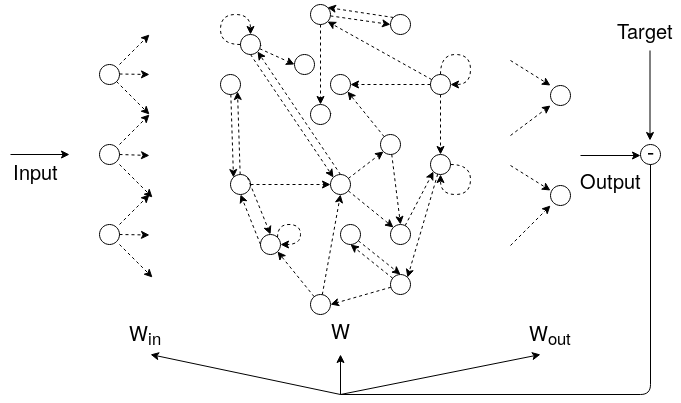
\includegraphics[width=0.7\linewidth]{immagini/RNN(1).png}
	\caption{Metodo di allenamento basato  su discesa di gradiente che adatta tutti i pesi delle connessioni.}
	\label{fig:RNN}
\end{figure} 

Le reti neurali ricorrenti si presentano come strumenti molto promettenti per elaborare sequenze temporali non lineari per due ragioni. Innanzitutto rappresentano una approssimazione dei sistemi dinamici, in secondo luogo si avvicinano al modello del cervello biologico grazie alle connessioni ricorrenti.\\
Tuttavia vi sono delle problematiche legate all'apprendimento evidenziate in \cite{RCapproch:paper} e riportate qui di seguito:
\begin{itemize}
	\item Non può essere garantita la convergenza del metodo di allenamento a discesa di gradiente, vi sono dei punti in cui le informazioni sul gradiente possono essere mal definite.
	\item L'aggiornamento di un solo parametro può essere computazionalmente costoso,
	cioè possono essere necessari molti cicli di aggiornamento. Questo comporta lunghi tempi di addestramento che rendono le RNN modelli convenienti utilizzando solo poche unità.
	\item È molto difficile apprendere relazioni che richiedono molta memoria perché le informazioni fornite dal gradiente subiscono una dissolvenza esponenziale nel tempo.
	\item  Gli algoritmi di apprendimento necessitano di  profonde conoscenze ed esperienza per essere applicati con successo.
\end{itemize}
In questa situazione di lento progresso, nel 2001 un nuovo approccio al design e all'allenamento delle RNN, noto come \textit{Reservoir Computing}, venne proposto indipendentemente da Wolfgang Maass \cite{w} e da Herbert Jaeger \cite{h}.





